% !TeX root = ../main.tex

\chapter{Keyword \& Category Decomposition}

We further analyze what category each spike captured, and what words contributes to those GPR index rise. The top 10 frequency words contributes to out GPR index spikes are: 統一、抗議、總統大選、聯合國、譴責、軍演、台獨、共軍、兩岸關係、解放軍. While top 10 words for Lau's GPR index are: 開始、發生、發展、準備、風險、爆發、啟動、危險、威脅、危機. It shows that those general verb may capture too many noise, which explains why our dictionary give more balanced category contribution percentage and less article selected.

\begin{figure}[htbp]
  \centering
  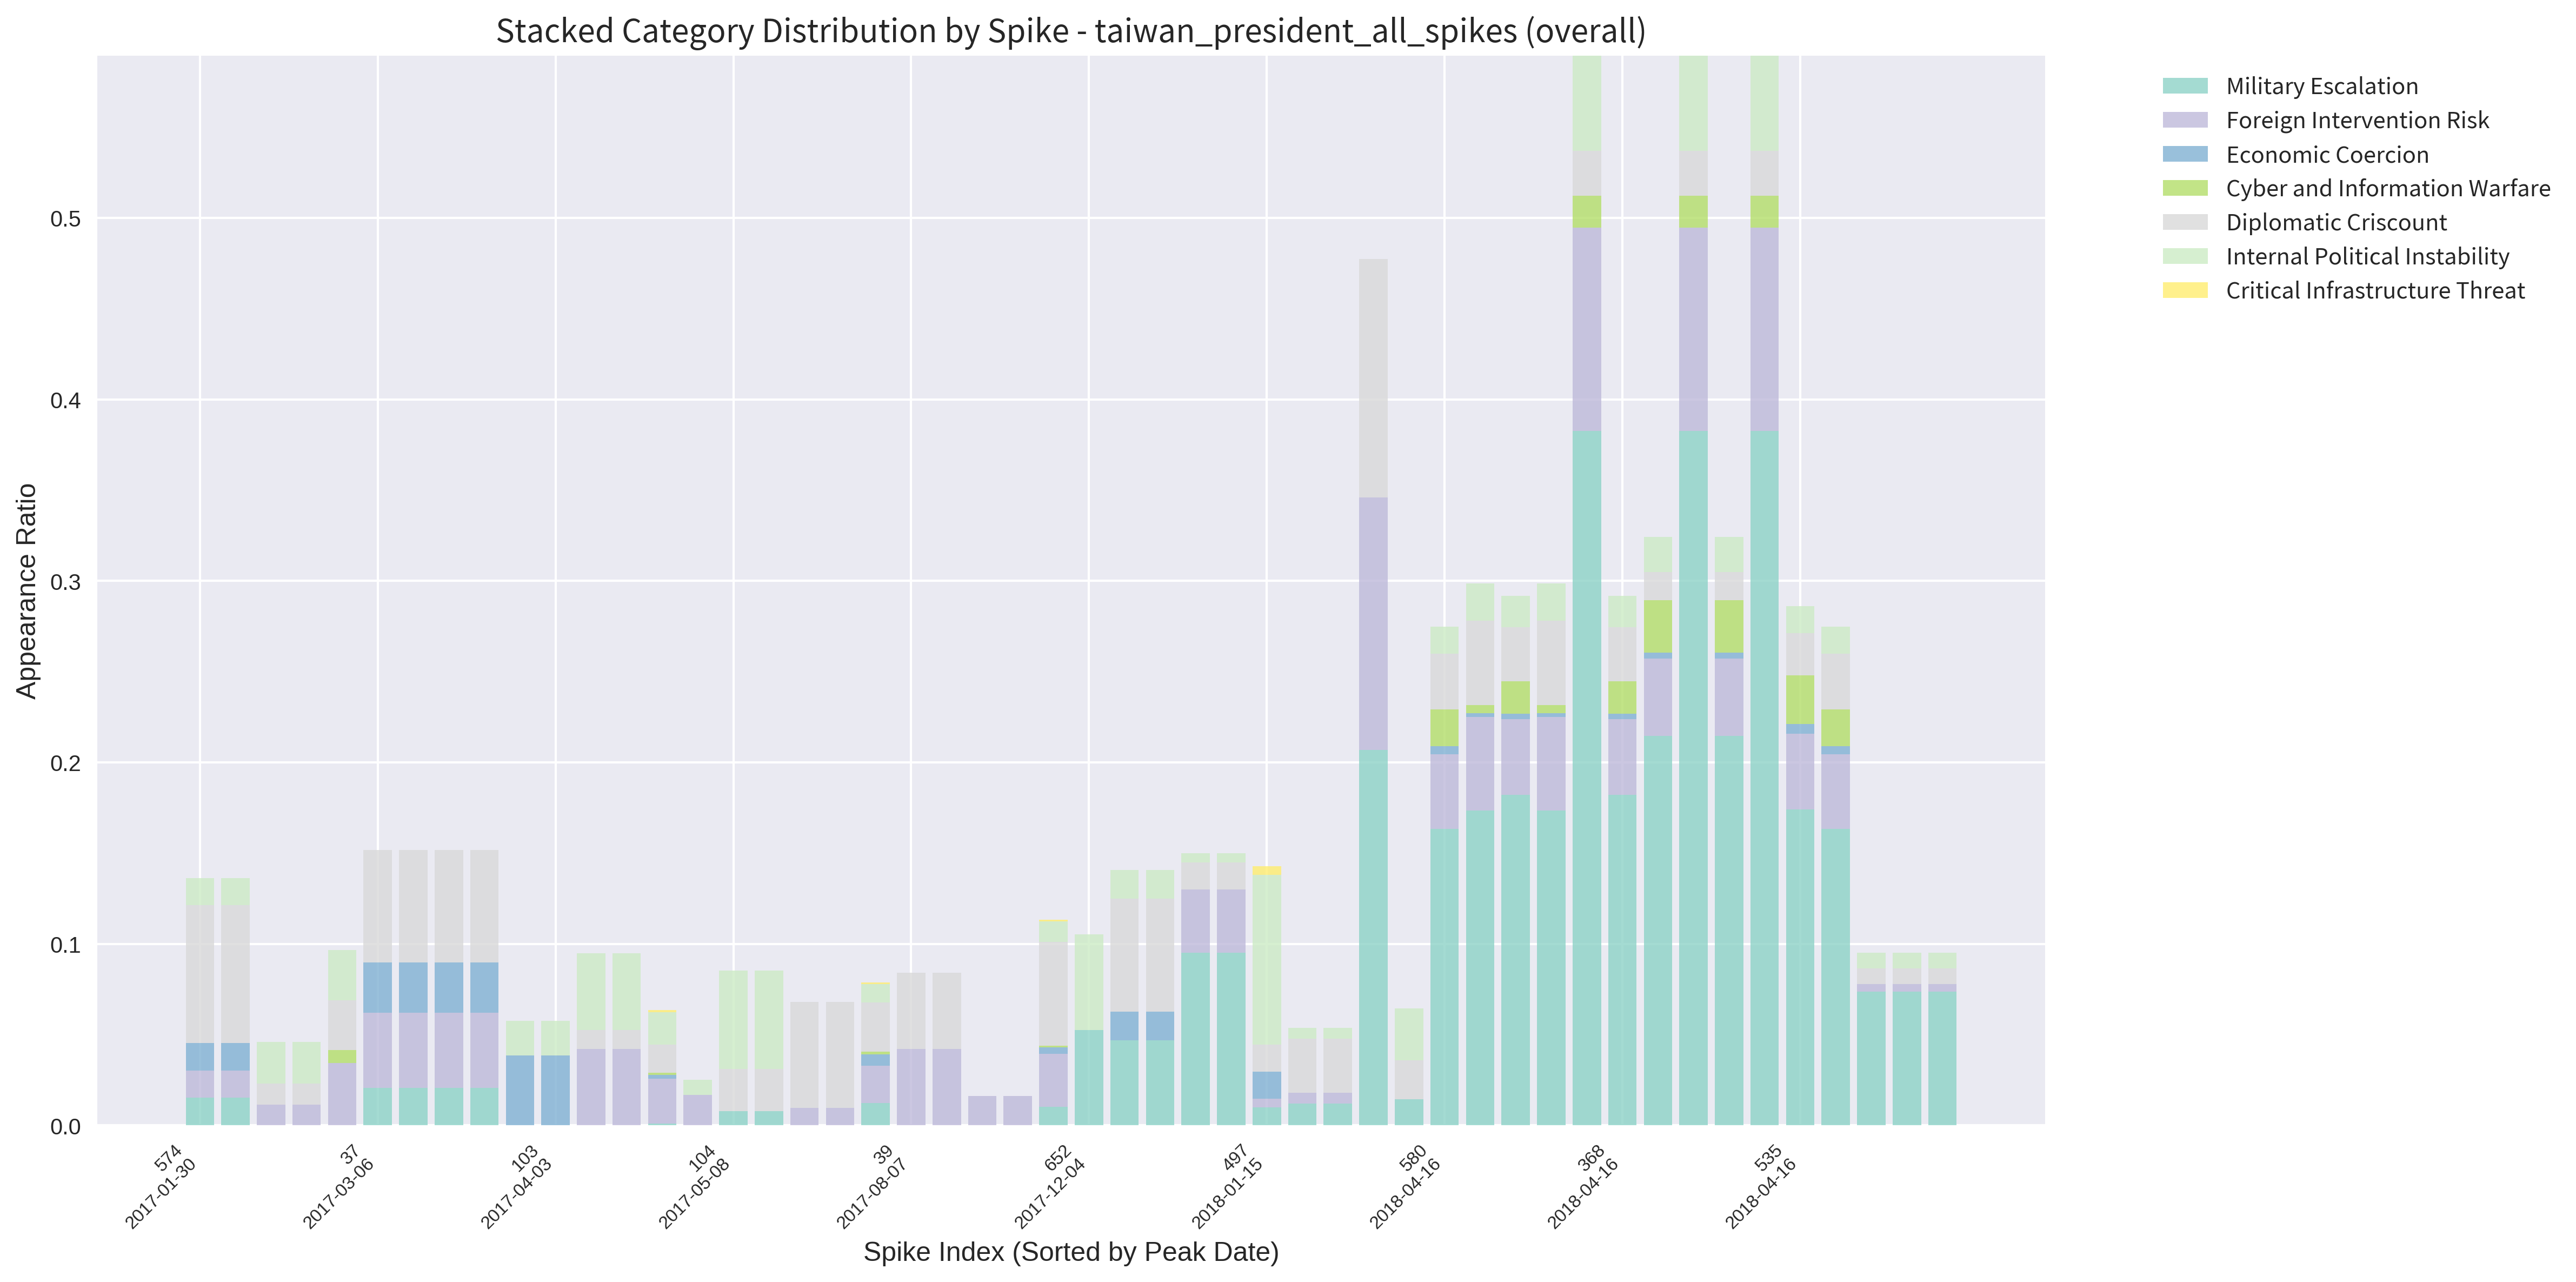
\includegraphics[width=\linewidth]{categories_stacked_taiwan_president_all_spikes.png}
  \caption{Proportion of each category for each spikes}
  \label{fig:my_example}
\end{figure}